\chapter{التقلص العضلي والوظيفة الحركية}\label{ch:b2:muscle-movement}

تغادر عدّاءة المكعبات بقوة على المضمار قدرها ثلاثة
أمثال وزنها، تولّدها في خُمس ثانية عضلات كانت
مرتخية قبل لحظة. ولم يقصر شيء في الخلية ليفعل
ذلك: بل انزلقت الخيوط في الداخل بعضها بجانب بعض، تجرها ملايين
الأيدي الجزيئية، كل منها يخطو خطوة عشرة نانومترات ثم يفلت،
عشر مرات في الثانية، بثمن ATP واحد في كل مرة. وهذا الفصل
يأخذ \omterm{def:b2:cell-differentiation:myogenesis}{الليفة العضلية} المبنية في \cref{ch:b2:cell-differentiation}
ويشغّلها: \omterm{prop:b2:muscle-movement:sliding}{انزلاق الخيوط} والمحرك الذي
يسوقها، ومفتاح الكالسيوم الذي يشغّل المحرك ويطفئه،
والأمر الآتي من العصب، وميكانيكا القوة والسرعة،
وكيف تدرّج الجملة العصبية الكل من \omterm{def:b2:muscle-movement:motorunit}{رعشة} إلى
عَدْو سريع.

\section{الخيوط المنزلقة}

\begin{proposition}[آلية انزلاق الخيوط]\label{prop:b2:muscle-movement:sliding}
\index{انزلاق الخيوط}\index{قسيم عضلي!التقلص}
حين تقصر \omterm{def:b2:cell-differentiation:myogenesis}{ليفة عضلية} تقصر قسيماتها العضلية
(\cref{ch:b2:cell-differentiation})، لكن لا خيوط الميوزين الغليظة
ولا خيوط الأكتين الرفيعة تغير طولها: فالخيوط الرفيعة
تنزلق إلى الداخل على امتداد الغليظة، ويضيق النطاق I والمنطقة
H، ويتقارب قرصا Z. والتداخل بين مجموعتي
الخيوط هو حيث تتولد القوة، ويولّد \omterm{def:b2:cell-differentiation:fibre}{القسيم العضلي}
قوة بنسبة التداخل: فمن طول ممطط قدره
\qty{3.6}{\micro m}، بلا تداخل ولا قوة، ترتفع
القوة خطيًا كلما تداخلت الخيوط أكثر، وتبلغ
مرتفعًا مستويًا قرب \qty{2.2}{\micro m} حيث يواجه كل رأس ميوزين أكتينًا،
ثم تهبط من جديد دون \qty{2.0}{\micro m} إذ تتصادم الخيوط الرفيعة
وتصطدم الغليظة بقرصي Z. وطول الراحة لعضلة
في الجسم يقع على المرتفع المستوي --- وهي أول إشارة
إلى كيف تُصنع القوة.
\end{proposition}
\begin{proof}[شواهد]
قاس أ.~ف.~هكسلي ونيدرغيركه، وه.~إ.~هكسلي وهانسون (1954)،
نطاقات ليفات مفردة ولييفات عضلية معزولة
بالتداخل وبمجهر الطور وهي تقصر: فحفظ النطاق A
طوله، وانكمش النطاق I، إذن فالخيوط تنزلق. وأمسك غوردون
وهكسلي وجوليان (1966) ليفة مفردة عند أطوال معينة بجهاز
ذي تغذية راجعة يُبقي طول \omterm{def:b2:cell-differentiation:fibre}{القسيم العضلي} في قطعة واحدة ثابتًا،
فوجدوا القوة متناسبة مع تداخل الخيوط الغليظة
والرفيعة المقيس بالمجهر الإلكتروني --- وهو منحني الطول والتوتر
بمرتفعه المستوي وذراعيه الخطيين، تمامًا كما تتنبأ هندسة
الخيوط.
\end{proof}

\begin{omfigure}
\begin{minipage}[b]{0.5\linewidth}\centering
\begin{tikzpicture}[every node/.style={font=\scriptsize}]
  \foreach \y/\lab/\ov in {2.4/{مرتخٍ، \qty{2.6}{\micro m}}/0.9, 1.2/{متقلص، \qty{2.0}{\micro m}}/0.3} {
    \begin{scope}[yshift=\y cm]
      \draw[very thick, omThm] (0,-0.35) -- (0,0.35); \draw[very thick, omThm] (4.4-2*\ov+1.0,-0.35) -- (4.4-2*\ov+1.0,0.35);
      \pgfmathsetmacro{\len}{4.4-2*\ov+1.0}
      \foreach \dy in {-0.25,0.05,0.25} { \draw[thick, omDef] (0,\dy) -- (1.5,\dy); \draw[thick, omDef] (\len,\dy) -- (\len-1.5,\dy); }
      \draw[line width=3pt, omExo!80!black] (\len/2-1.1,-0.1) -- (\len/2+1.1,-0.1);
      \node[right] at (\len+0.15,0) {\lab};
    \end{scope}
  }
  \node[align=center] at (2.7,0.1) {تحفظ الخيوط أطوالها؛\\ويكبر التداخل إذ يتقارب قرصا Z};
\end{tikzpicture}
\end{minipage}\hfill
\begin{minipage}[b]{0.48\linewidth}\centering
\begin{tikzpicture}
\begin{axis}[
  width=\linewidth, height=4.8cm,
  axis x line=bottom, axis y line=left,
  xmin=1.2, xmax=3.8, ymin=0, ymax=1.15,
  xlabel={طول القسيم العضلي (\unit{\micro m})}, ylabel={القوة (نسبيًا)},
  xlabel style={font=\scriptsize, at={(axis description cs:0.5,-0.17)}, anchor=north},
  ylabel style={font=\scriptsize},
  tick label style={font=\scriptsize}, xtick={1.3,2.0,2.2,3.6}, ytick={0,0.5,1},
  clip=false,
]
\addplot[very thick, omDef] coordinates {(1.3,0) (1.65,0.5) (2.0,1) (2.2,1) (3.6,0)};
\node[font=\scriptsize, anchor=south] at (axis cs:2.1,1.02) {المرتفع المستوي};
\node[font=\scriptsize, anchor=west, align=left] at (axis cs:2.95,0.75) {التداخل\\يتناقص};
\end{axis}
\end{tikzpicture}
\end{minipage}

{\small إلى اليسار: \omterm{def:b2:cell-differentiation:fibre}{قسيم عضلي} مرتخٍ ومتقلص --- الخيوط
الرفيعة (الزرقاء) تنزلق على امتداد الغليظة (الرمادية) دون تغير
طولها. وإلى اليمين: منحني الطول والتوتر: فالقوة متناسبة مع
التداخل، وأعظم ما تكون على المرتفع المستوي حيث تستريح العضلة.}
\end{omfigure}

\begin{omfigure}
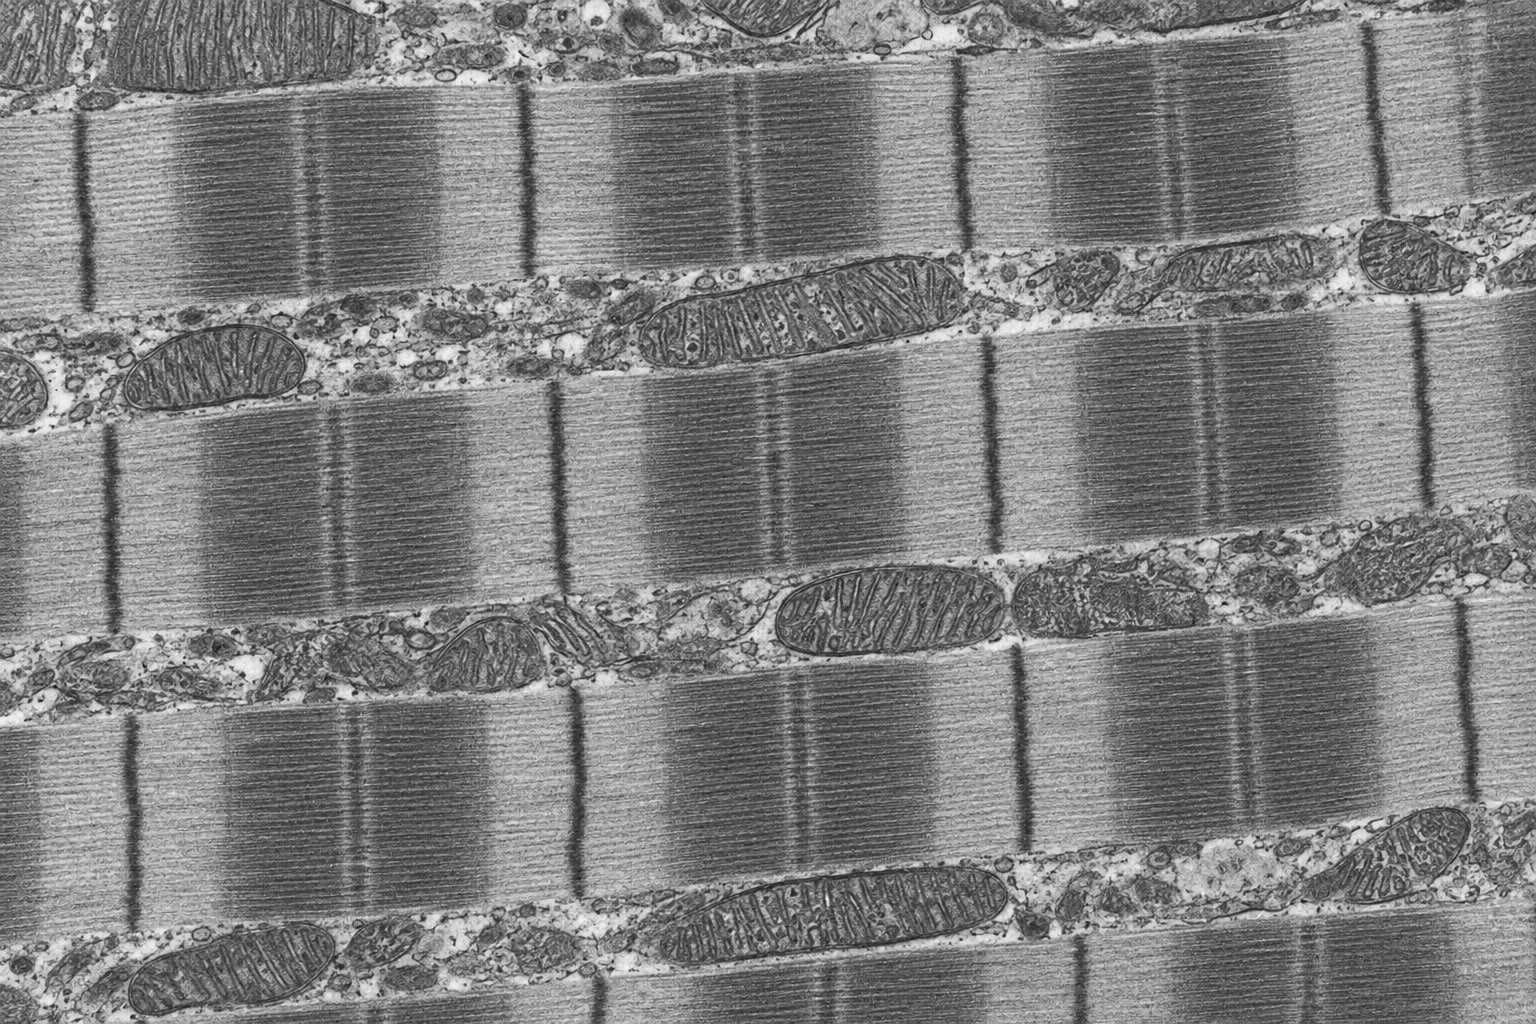
\includegraphics[width=0.6\linewidth]{images/book4/ai/b4-21-sarcomere-tem.jpg}

{\small لييفات عضلية تحت المجهر الإلكتروني: نطاقات A من
الخيوط الغليظة، ونطاقات I من الخيوط الرفيعة تنصّفها خطوط Z،
والمتقدرات بين اللييفات التي تدفع ثمن الانزلاق.}
\end{omfigure}

\section{المحرك}

\begin{proposition}[دورة الجسر المستعرض]\label{prop:b2:muscle-movement:crossbridge}
\index{دورة الجسر المستعرض}\index{ميوزين}\index{ATP!في التقلص}
يشرئب من كل خيط غليظ نحو ثلاثمئة \emph{رأس
ميوزين}، وكل رأس محرك يمشي على امتداد الأكتين في دورة
من أربع خطوات. (1) فإذا ارتبط به ATP كان الرأس منفصلًا عن الأكتين؛
ويحلم ATP إلى ADP وفوسفات ويتزنبرك في
شكل مشدود عالي الطاقة. (2) ثم يرتبط الرأس المزنبرك بوحيدة أكتين،
فيتألف \emph{جسر مستعرض}. (3) ثم يُطلق الفوسفات
فينقلب الرأس إلى شكله المرتخي، جارًّا الخيط الرفيع
نحو \qty{10}{nm} نحو مركز \omterm{def:b2:cell-differentiation:fibre}{القسيم العضلي} --- وهي
\emph{ضربة القدرة}؛ ويغادر ADP. (4) ثم يرتبط ATP جديد فيفلت الرأس
الأكتينَ؛ ودون ATP لا يستطيع الإفلات، وهو تصلب
الموت. وتستغرق الدورة نحو جزء من عشرين من الثانية؛ ويقضي الرأس
معظمها منفصلًا، حتى لا يجر في أي لحظة إلا كسر
من الرؤوس، ولا يُترك خيط منزلق بسرعة قط.
والقوة مجموع جذبات الرؤوس المرتبطة؛ والتقصير
مجموع خطواتها، وهو نصف ميكرومتر لكل \omterm{def:b2:cell-differentiation:fibre}{قسيم عضلي} في الدورة
على الأكثر؛ والطاقة ATP واحد لكل خطوة لكل رأس، أي نحو
\qty{50}{kJ/mol} --- و\qty{8e-20}{J} لكل خطوة، يحوّل الرأس
منها إلى شغل ما يصل إلى النصف.
\end{proposition}

\begin{omfigure}
\begin{tikzpicture}[every node/.style={font=\scriptsize}, >=stealth]
  \foreach \x/\lab/\ang/\att in {0/{1. ارتباط ATP:\\انفصال؛ وحلمهة\\ATP وزنبرة الرأس}/60/0, 3.6/{2. الرأس المزنبرك\\يرتبط بالأكتين:\\جسر مستعرض}/60/1, 7.2/{3. إطلاق الفوسفات:\\ضربة القدرة،\\وجر الخيط \qty{10}{nm}}/20/1, 10.8/{4. مغادرة ADP وارتباط\\ATP جديد: الرأس\\يفلت}/20/0} {
    \begin{scope}[xshift=\x cm]
      \draw[thick, omDef] (0,2.2) -- (2.8,2.2); \foreach \i in {0.2,0.6,...,2.6} \fill[omDef!50] (\i,2.2) circle (0.14);
      \draw[line width=3pt, omExo!80!black] (0,0.4) -- (2.8,0.4);
      \draw[very thick, omThm] (1.4,0.4) -- (1.4,1.0);
      \ifnum\att=1 \draw[very thick, omThm] (1.4,1.0) -- ++(\ang:1.15); \fill[omThm] (1.4,1.0) ++(\ang:1.15) circle (0.16); \else \draw[very thick, omThm] (1.4,1.0) -- ++(\ang:1.0); \fill[omThm] (1.4,1.0) ++(\ang:1.0) circle (0.16); \fi
      \node[below, align=center] at (1.4,0.15) {\lab};
    \end{scope}
  }
  \draw[->, thick, omDef] (7.9,2.55) -- (8.9,2.55); \node[omDef, above] at (8.4,2.6) {الخيط الرفيع يتحرك};
\end{tikzpicture}

{\small \omterm{prop:b2:muscle-movement:crossbridge}{دورة الجسر المستعرض}. رأس ميوزين مزنبرك (أحمر) يرتبط
بالأكتين (أزرق)، ويطلق الفوسفات ويجر الخيط الرفيع عبر
ضربة قدرته، ثم يرتبط بجزيء ATP جديد فيفلت.}
\end{omfigure}

\begin{theorem}[قوة العضلة وسرعتها واستطاعتها]\label{thm:b2:muscle-movement:hill}
\index{منحني القوة والسرعة}\index{استطاعة عضلية}
تهبط قوة العضلة كلما قصرت أسرع، لأن الخيوط كلما
انزلقت أسرع قلّ عدد الرؤوس المرتبطة في أي لحظة
وكثر ما يُجَرّ منها بعد ضربته قبل أن
يفلت. وعلاقة هِل تصف ذلك:
\[
(F + a)(v + b) = (F_0 + a)\,b,
\]
حيث $F_0$ القوة متساوية القياس (عند $v = 0$)، و$v_{\max} =
F_0 b/a$ السرعة بلا حمل، و$a$ و$b$ ثابتان ($a \approx
F_0/4$). والاستطاعة $Fv$ صفر عند الطرفين وأعظم ما تكون عند نحو
ثلث $v_{\max}$ وثلث $F_0$ --- ولذلك يبدّل راكب الدراجة
ترسه ويكون لخطوة العدّاءة معدل مفضل. وتولّد عضلة
الإنسان نحو \qty{30}{N} في كل سنتيمتر مربع من
المقطع، وتقصر إلى عشرة أطوال في الثانية، وتسلّم
نحو \qty{100}{W} في الكيلوغرام في أحسن حالاتها.
\end{theorem}
\begin{proof}
منحني هِل تجريبي (1938)، قيس على عضلة ضفدع معزولة
بوصفه سرعة التقصير في مقابل الحمل الذي ترفعه؛ ويلائمه القطع الزائد
لأن كسر الرؤوس المرتبطة يهبط مع سرعة الانزلاق
وقوة كل رأس مرتبط تهبط إذ يُحمل عبر
ضربته. والاستطاعة: مع $F = (F_0 + a)b/(v + b) - a$، تكون $Fv$ صفرًا عند
$v = 0$ وعند $v_{\max}$؛ والاشتقاق يعطي الأعظم عند
$v = b(\sqrt{(F_0 + a)/a} - 1)$، وهو عند $a = F_0/4$ يساوي $v =
1.24\,b = 0.31\,v_{\max}$، حيث $F = 0.31\,F_0$.
\end{proof}

\begin{omfigure}
\begin{tikzpicture}
\begin{axis}[
  width=0.7\linewidth, height=5.4cm,
  axis x line=bottom, axis y line=left,
  xmin=0, xmax=1.05, ymin=0, ymax=1.1,
  xlabel={سرعة التقصير $v/v_{\max}$}, ylabel={القوة $F/F_0$ والاستطاعة (نسبيًا)},
  xlabel style={font=\small, at={(axis description cs:0.5,-0.13)}, anchor=north},
  ylabel style={font=\small},
  tick label style={font=\small}, xtick={0,0.31,1}, xticklabels={0,0.31,1}, ytick={0,0.31,1}, yticklabels={0,0.31,1},
  legend style={font=\scriptsize, at={(0.97,0.95)}, anchor=north east, draw=none},
  clip=false,
]
\addplot[very thick, omDef, domain=0:1, samples=100] {(1.25*0.25)/(x+0.25) - 0.25};
\addlegendentry{القوة}
\addplot[very thick, omThm, domain=0:1, samples=100] {10.4*x*((1.25*0.25)/(x+0.25) - 0.25)};
\addlegendentry{الاستطاعة (مقيسة)}
\draw[dashed, gray] (axis cs:0.31,0) -- (axis cs:0.31,1.0);
\end{axis}
\end{tikzpicture}

{\small منحني هِل للقوة والسرعة ($a = F_0/4$) والاستطاعة التي
يقتضيها: فالقوة تهبط كلما قصرت العضلة أسرع، والاستطاعة تبلغ الذروة
عند نحو ثلث السرعة القصوى وثلث القوة متساوية
القياس.}
\end{omfigure}

\section{المفتاح: الكالسيوم}

\begin{proposition}[الاقتران بين الاستثارة والتقلص]\label{prop:b2:muscle-movement:coupling}
\index{اقتران الاستثارة والتقلص}\index{تروبونين}\index{تروبوميوزين}\index{شبكة هيولية عضلية}
في الراحة لا تستطيع رؤوس الميوزين بلوغ الأكتين: فمواقع الارتباط
على الخيط الرفيع يغطيها \emph{التروبوميوزين}، وهو قضيب يرقد
في ثلم حلزون الأكتين، يمسكه هناك \emph{التروبونين}.
والمفتاح هو الكالسيوم. فكمون فعل على غشاء الليفة
يجري نازلًا في نبيبات T إلى الداخل، وعند الوصلات
التي يلاقي فيها \omterm{def:b2:cell-differentiation:fibre}{نبيب T} الشبكةَ الهيولية العضلية، يفتح
قنوات إطلاق الكالسيوم في الشبكة؛ فيغمر الكالسيوم اللييفات العضلية،
مرتفعًا من \qty{0.1}{} إلى \qty{10}{\micro mol/L} في مليثانية،
ويرتبط بالتروبونين، فيزيح التروبونين التروبوميوزين عن مواقع
الارتباط: فترتبط الرؤوس، وتتقلص الليفة ما دام
الكالسيوم. ثم تعيد مضخات في الشبكة، تحرق ATP،
الكالسيوم في غضون عشرات المليثوان؛ فيعود التروبوميوزين يغطي
المواقع وترتخي الليفة. فالارتخاء إذن فعال كالتقلص،
والعضلة المحرومة من ATP لا تستطيع إفلات
رؤوسها ولا ضخ كالسيومها --- وهو التصلب الرمّي. وفي \omterm{def:b2:heart:anatomy}{القلب} يُستعمل المفتاح
نفسه، لكن بكالسيوم يدخل من الخارج عبر
قنوات الغشاء نفسه ليطلق الإطلاق، ولذلك كان
\omterm{def:b2:heart:anatomy}{القلب}، لا العضل الهيكلي، حساسًا لكالسيوم
الدم.
\end{proposition}

\begin{omfigure}
\begin{tikzpicture}[every node/.style={font=\scriptsize}, >=stealth]
  \node[draw, rounded corners, fill=omDef!15, align=center] (nerve) at (0,0) {دفعة العصب\\الحركي};
  \node[draw, rounded corners, fill=omDef!15, align=center] (nmj) at (3.0,0) {الوصل العصبي\\العضلي:\\أستيل كولين};
  \node[draw, rounded corners, fill=omDef!15, align=center] (ap) at (6.2,0) {كمون فعل عضلي،\\نازلًا في\\نبيبات T};
  \node[draw, rounded corners, fill=omThm!15, align=center] (ca) at (9.4,0) {إطلاق Ca$^{2+}$\\من الشبكة الهيولية\\العضلية};
  \node[draw, rounded corners, fill=omProp!20, align=center] (tn) at (12.6,0) {التروبونين يرتبط بشاردة Ca$^{2+}$،\\والتروبوميوزين يتزحزح،\\والرؤوس ترتبط};
  \node[draw, rounded corners, fill=omExo!25, align=center] (off) at (9.4,-2.2) {المضخات تعيد Ca$^{2+}$ (بإنفاق ATP)؛\\والتروبوميوزين يغطي الأكتين:\\ارتخاء};
  \draw[->, thick] (nerve) -- (nmj); \draw[->, thick] (nmj) -- (ap); \draw[->, thick] (ap) -- (ca); \draw[->, thick] (ca) -- (tn);
  \draw[->, thick] (ca) -- (off);
  \node[below, gray] at (1.5,-0.7) {\qty{0.6}{ms}}; \node[below, gray] at (4.6,-0.7) {\qty{1}{ms}}; \node[below, gray] at (7.8,-0.7) {\qty{1}{ms}};
\end{tikzpicture}

{\small من دفعة العصب إلى القوة: الوصل، وكمون فعل الليفة
نفسها، وإطلاق الكالسيوم، وكشف مواقع
الأكتين --- ثم المضخات التي تنهي ذلك.}
\end{omfigure}

\section{الأمر والتدريج}

\begin{definition}[الوحدة الحركية]\label{def:b2:muscle-movement:motorunit}
\index{وحدة حركية}\index{رعشة}\index{كزاز}\index{تجنيد}
يرسل \emph{\omterm{def:b2:neurons-synapses:neuron}{العصبون} الحركي} في النخاع الشوكي محواره إلى
عضلة ويتفرع ليعصّب من حفنة إلى ألف
ليفة، مبعثرة في العضلة؛ \omterm{def:b2:neurons-synapses:neuron}{والعصبون} وليفاته
\emph{وحدة حركية}، وهي أصغر كمية قوة تستطيع الجملة
العصبية أن تأمر بها. وكل دفعة في \omterm{def:b2:neurons-synapses:neuron}{العصبون} تجعل كل ليفة
في الوحدة تنطلق مرة وتعطي \emph{رعشة}: أي قوة ترتفع
في نحو \qty{30}{ms} وتخبو في \qty{100}{ms}، لأن
دفقة الكالسيوم قصيرة. والدفعات في تعاقب سريع تجعل الرعشات
تتجمع، إذ لم يكن كالسيوم إحداها قد ضُخّ بعيدًا حين تصل
التالية؛ وعند نحو 30 إلى 50 دفعة في الثانية تندمج القوة
في \emph{كزاز} أملس، يبلغ ثلاثة إلى خمسة أمثال الرعشة.
وتدرّج الجملة العصبية قوة العضلة بطريقتين: \emph{بالمعدل}
الذي تنطلق به كل وحدة، و\emph{بعدد}
الوحدات التي تجنّدها --- فالوحدات الصغيرة البطيئة المقاومة للتعب أولًا
(وهو \emph{مبدأ الحجم})، والكبيرة السريعة آخرًا، ولا تكون إلا لأشد
الجهود. ومن ثم فالعضلة في الاستعمال العادي ليست مشتغلة
كلها قط: بل ينطلق كسر من وحداتها، بالتناوب، ويستريح الباقي.
\end{definition}

\begin{omfigure}
\begin{tikzpicture}
\begin{axis}[
  width=0.82\linewidth, height=5.4cm,
  axis x line=bottom, axis y line=left,
  xmin=0, xmax=1.0, ymin=0, ymax=4.2,
  xlabel={الزمن (s)}, ylabel={القوة (الرعشة $=$ 1)},
  xlabel style={font=\small, at={(axis description cs:0.5,-0.13)}, anchor=north},
  ylabel style={font=\small},
  tick label style={font=\small}, xtick={0,0.2,0.4,0.6,0.8,1}, ytick={0,1,2,3,4},
  clip=false,
]
% single twitch
\addplot[very thick, omDef, domain=0:0.2, samples=60] {(x<0.02)*0 + (x>=0.02)*4.5*(x-0.02)*exp(-(x-0.02)/0.03)*4.1};
% summation at 10 Hz
\addplot[very thick, omProp, domain=0.25:0.62, samples=200] {(x>=0.25)*4.5*4.1*(x-0.25)*exp(-(x-0.25)/0.03) + (x>=0.33)*4.5*4.1*(x-0.33)*exp(-(x-0.33)/0.03) + (x>=0.41)*4.5*4.1*(x-0.41)*exp(-(x-0.41)/0.03) + (x>=0.49)*4.5*4.1*(x-0.49)*exp(-(x-0.49)/0.03)};
% tetanus at 50 Hz
\addplot[very thick, omThm, domain=0.66:0.98, samples=100] {3.8*(1-exp(-(x-0.66)/0.06))};
\node[font=\scriptsize, anchor=west] at (axis cs:0.09,0.7) {دفعة واحدة: رعشة};
\node[font=\scriptsize, anchor=south] at (axis cs:0.44,2.2) {\qty{12}{Hz}: تجميع};
\node[font=\scriptsize, anchor=south] at (axis cs:0.82,3.85) {\qty{50}{Hz}: كزاز مندمج};
\end{axis}
\end{tikzpicture}

{\small تدريج القوة بالمعدل. الدفعة الواحدة تعطي \omterm{def:b2:muscle-movement:motorunit}{رعشة}؛
والدفعات باثنتي عشرة في الثانية تتجمع في قوة متموجة؛ وعند خمسين في
الثانية تندمج القوة في \omterm{def:b2:muscle-movement:motorunit}{كزاز} يبلغ أمثال \omterm{def:b2:muscle-movement:motorunit}{الرعشة}.}
\end{omfigure}

\begin{proposition}[المنعكسات والنخاع الشوكي]\label{prop:b2:muscle-movement:reflex}
\index{قوس منعكس}\index{مغزل عضلي}\index{منعكس التمطط}\index{تثبيط متبادل}
\omterm{def:b2:neurons-synapses:neuron}{العصبون} الحركي هو \emph{الطريق النهائي المشترك}: فكل أمر،
من القشر أو من منعكس، ينتهي عليه. وأبسط دارة
هي \emph{\omterm{prop:b2:muscle-movement:reflex}{منعكس التمطط}} في \cref{ch:b2:neurons-synapses}:
فالنهايات الحسية الملفوفة حول ليفات خاصة داخل العضلة،
وهي \emph{المغازل العضلية}، تنطلق حين تُمطط العضلة، فتهيّج
العصبونات الحركية للعضلة نفسها عبر \omterm{def:b2:neurons-synapses:synapse}{مشبك} واحد، وتثبط
عصبونات المضاد عبر \omterm{def:b2:neurons-synapses:neuron}{عصبون} بيني
(وهو \emph{\omterm{prop:b2:muscle-movement:reflex}{التثبيط المتبادل}})، فتقاوم العضلة
التمطط --- وهو أساس القوام، إذ كل ترنح تمطط
لعضلة ما. ومستقبل ثانٍ، وهو عضو الوتر، ينطلق حين تكون
قوة العضلة عالية فيثبط عصبوناتها الحركية: أي صمام
أمان. والسحب من منبه مؤلم منعكس من عدة
مشابك يعطف الطرف، ويبسط، على الجهة الأخرى،
الطرفَ الآخر حتى لا تقع. والدماغ لا يأمر
العضلات بل الحركات: فالقشر يرسل خطة، والمخيخ
يصححها في مقابل ما تبلّغه المغازل، والعقد القاعدية
تطلقها، ودارات النخاع الشوكي، التي تستطيع إدارة
إيقاع الخطو وحدها، تنفّذها --- وهو موضوع
مجلد السنة الثالثة.
\end{proposition}

\begin{omfigure}
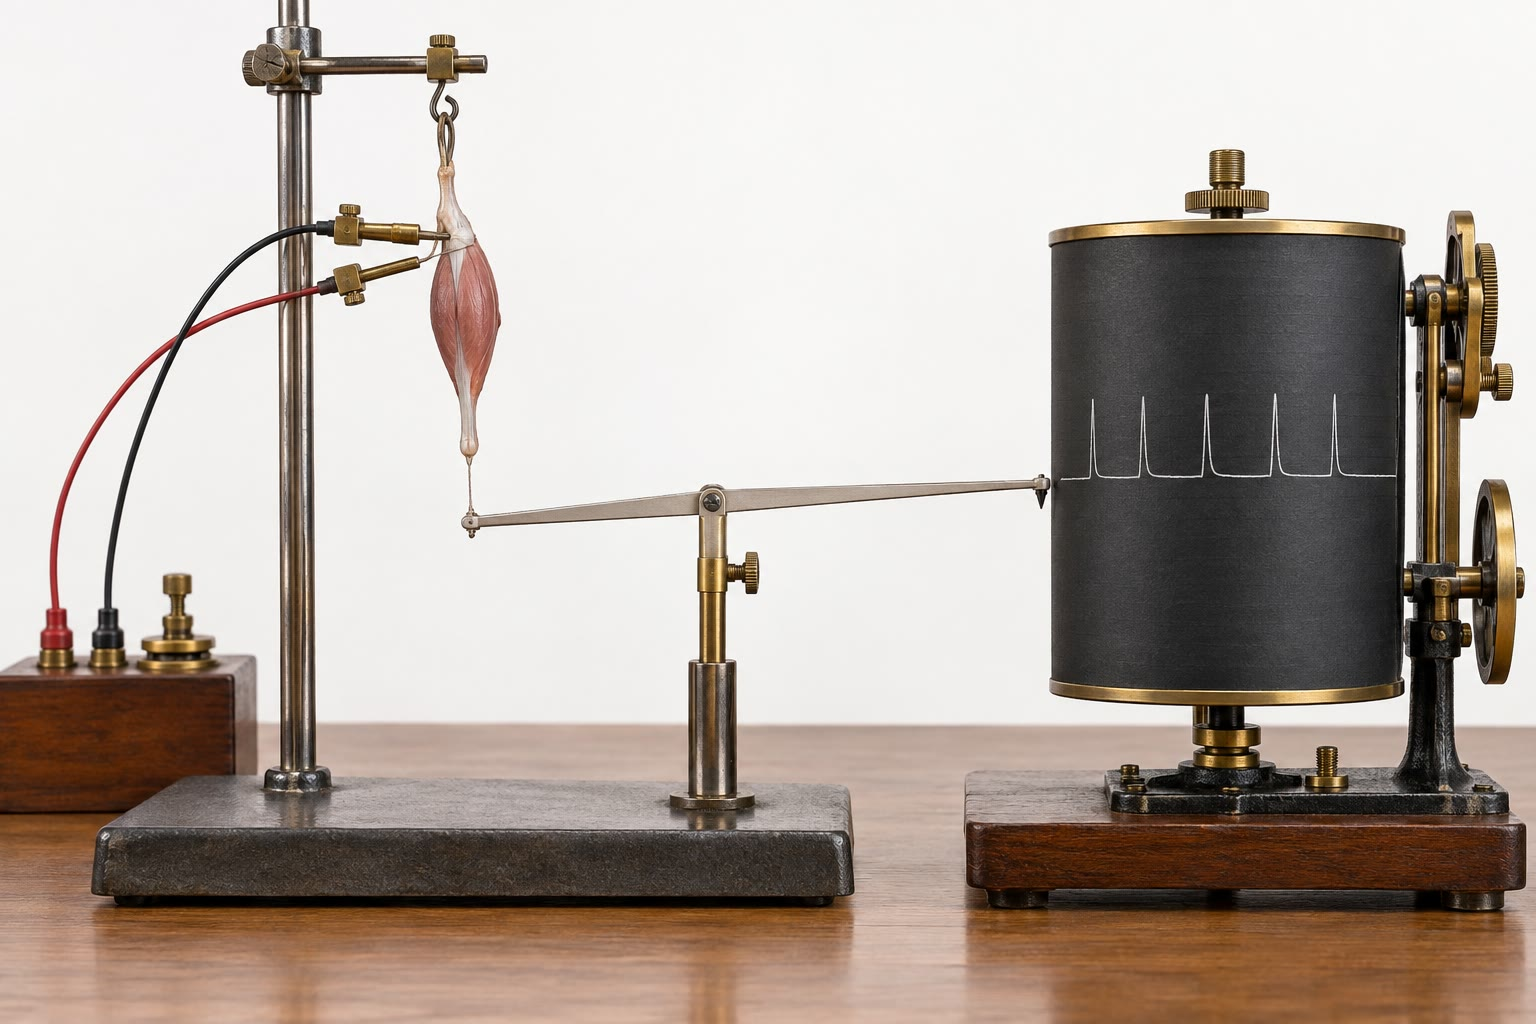
\includegraphics[width=0.44\linewidth]{images/book4/ai/b4-21-frog-muscle-prep.jpg}\hspace{0.04\linewidth}
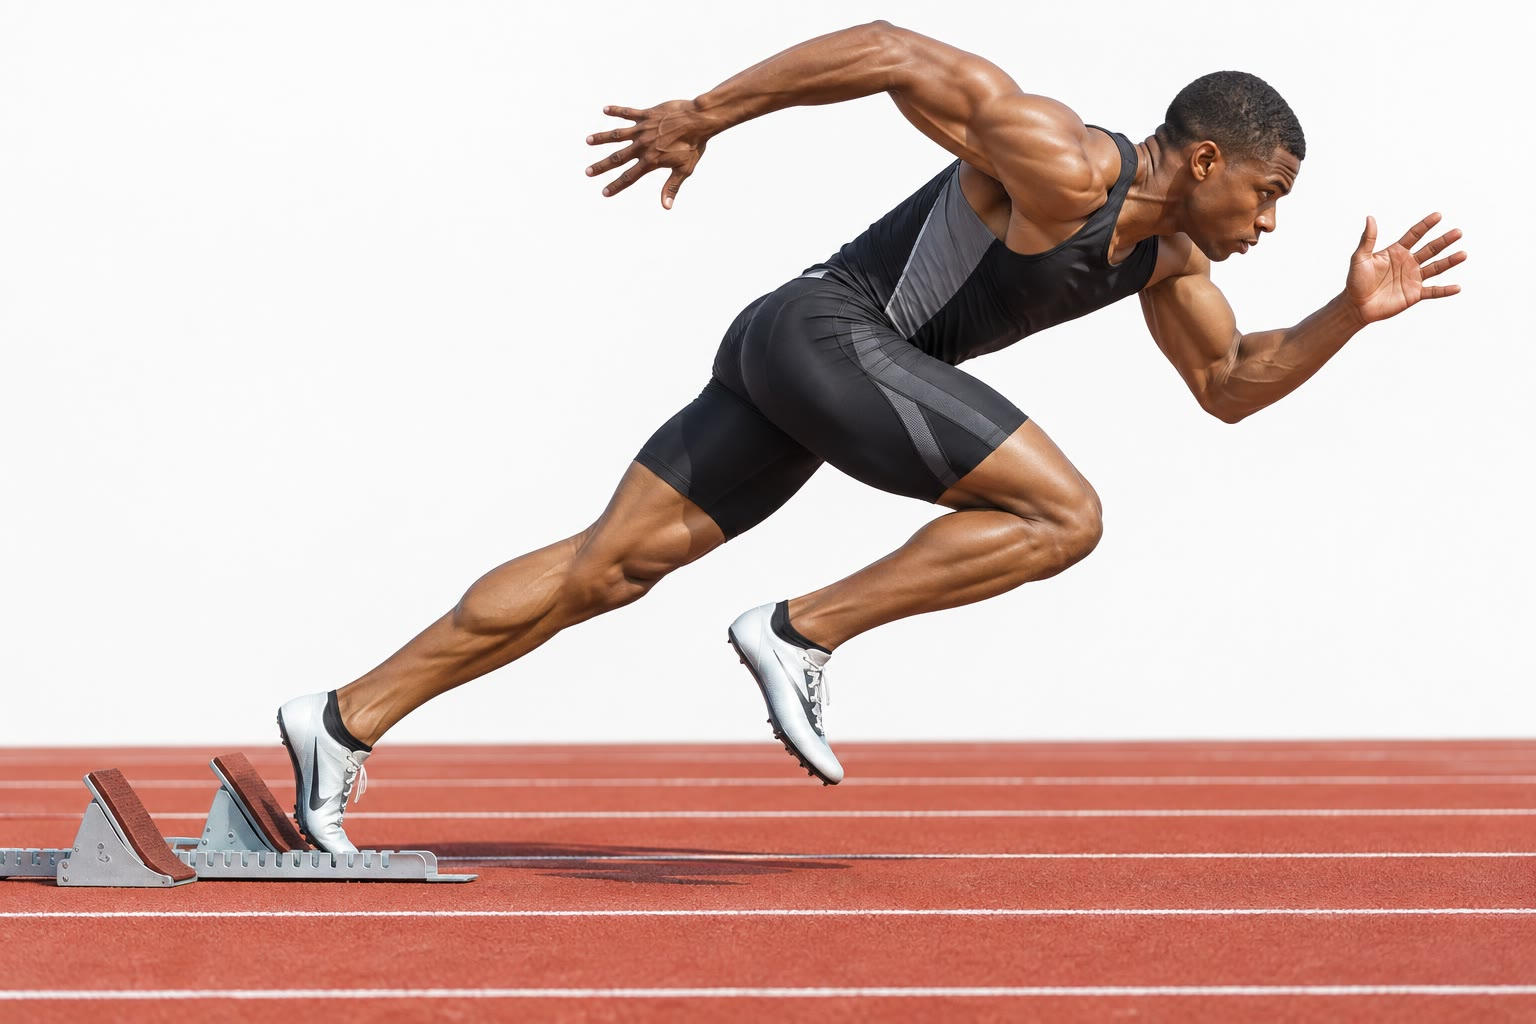
\includegraphics[width=0.44\linewidth]{images/book4/ai/b4-21-sprinter.jpg}

{\small إلى اليسار: التحضير الكلاسيكي --- عضلة ضفدع، مع
عصبها، وأقطاب التنبيه، وذراع يكتب على أسطوانة مدخَّنة
--- وعليه سُجّلت أول مرة \omterm{def:b2:muscle-movement:motorunit}{الرعشة} والتجميع \omterm{def:b2:muscle-movement:motorunit}{والكزاز}.
وإلى اليمين: الفيزيولوجيا نفسها في أقصى امتدادها.}
\end{omfigure}

\section{الوقود والتعب}

\begin{proposition}[دفع ثمن الشغل]\label{prop:b2:muscle-movement:energy}
\index{فوسفات الكرياتين}\index{تعب عضلي}\index{دين الأكسجين}
تحمل الليفة ATP يكفي ثانية أو ثانيتين من جهد كامل. والاحتياطي
الأول \emph{\omterm{prop:b2:muscle-movement:energy}{فوسفات الكرياتين}}، الذي يعيد فسفرة ADP
في غضون مليثوان ويدوم نحو عشر ثوانٍ --- وهو وقود العدّاءة.
والثاني \emph{التحلل السكري} لغليكوجين الليفة،
بلا أكسجين، ويعطي ATP اثنين لكل غلوكوز ولاكتات: وهو سريع،
يكفي دقيقة أو دقيقتين، ويحد نفسه إذ يتراكم الحمض والفوسفات.
والثالث الاستقلاب \emph{المؤكسِد} للغلوكوز
وللحموض الدسمة في المتقدرات، وهو ثلاثون ATP لكل غلوكوز، ولا يحده
إلا الأكسجين الذي يسلّمه الدم
(\cref{ch:b2:blood-pressure}): وهو الماراثون. فالليفات السريعة السكرية
تعتمد على الأولين وتتعب في دقيقة؛ والليفات البطيئة المؤكسِدة،
الحمراء بالميوغلوبين المحشوة بالمتقدرات، تجري ساعات.
و\emph{التعب} في جهد قصير ليس نفاد ATP ---
فذلك كان سيترك العضلة في تصلب --- بل تراكم
الفوسفات والبروتونات، وهي تضعف الجسور المستعرضة وإطلاق
الكالسيوم؛ وهو في جهد طويل نفاد الغليكوجين
ثم، في النهاية، نفاد الإرادة. وبعد الجهد تسدد العضلة
\emph{\omterm{prop:b2:muscle-movement:energy}{دين الأكسجين}}: فتعيد \omterm{prop:b2:muscle-movement:energy}{فوسفات الكرياتين}، وتحوّل
اللاكتات راجعةً (في الكبد)، وتملأ مخازنها، وهي تتنفس
بشدة دقائق بعد الوقوف ساكنة.
\end{proposition}

\begin{example}[مئة متر]\label{ex:b2:muscle-movement:sprint}
عشر ثوانٍ من جهد أقصى من \qty{20}{kg} من عضل الساقين عند
\qty{100}{W/kg} هي \qty{2}{kW} من الاستطاعة الميكانيكية، وعند
مردود \qty{25}{\%} تكون \qty{8}{kW} من دوران ATP --- أي نحو
\qty{160}{mmol} من ATP في الثانية، أو \qty{800}{g} من ATP في السباق.
وتحمل العضلة نحو خمسين غرامًا؛ ويمد \omterm{prop:b2:muscle-movement:energy}{فوسفات الكرياتين} الثواني الخمس
الأولى، ويمد التحلل السكري الباقي، وتنهي العدّاءة السباق و
اللاكتات عند \qty{15}{mmol/L} في دمها ودين تسدده على مدى
الربع ساعة التالي. أما عدّاء الماراثون عند \qty{300}{W} لساعتين
فيحرق \qty{2}{MJ} من الشغل، و\qty{8}{MJ} من الوقود --- أي كيلوغرامًا من
الغليكوجين والشحم --- مع أكسجين يُسلَّم عند \qty{4}{L/min} طوال
الطريق، والجدار الذي يصطدم به عند الكيلومتر الثلاثين هو قاع
غليكوجينه.
\end{example}

\section{تمارين}

\begin{exercise}[$\star$]\label{exo:b2:muscle-movement:1}
اذكر آلية \omterm{prop:b2:muscle-movement:sliding}{انزلاق الخيوط} وقل أي نطاقات
\omterm{def:b2:cell-differentiation:fibre}{القسيم العضلي} تتغير عند التقلص وأيها لا تتغير.
\end{exercise}

\begin{exercise}[$\star$]\label{exo:b2:muscle-movement:2}
أعطِ خطوات \omterm{prop:b2:muscle-movement:crossbridge}{دورة الجسر المستعرض} الأربع ودور ATP
في كل خطوة. ولماذا تتيبس عضلة بلا ATP؟
\end{exercise}

\begin{exercise}[$\star$]\label{exo:b2:muscle-movement:3}
اذكر الأحداث من دفعة العصب الحركي إلى ارتباط
رؤوس الميوزين، مع الزمن الذي يستغرقه كل حدث.
\end{exercise}

\begin{exercise}[$\star$]\label{exo:b2:muscle-movement:4}
عرّف \omterm{def:b2:muscle-movement:motorunit}{الوحدة الحركية} \omterm{def:b2:muscle-movement:motorunit}{والرعشة} \omterm{def:b2:muscle-movement:motorunit}{والكزاز}، وأعطِ الطريقتين اللتين
تدرّج بهما الجملة العصبية القوة.
\end{exercise}

\begin{exercise}[$\star\star$]\label{exo:b2:muscle-movement:5}
\omterm{def:b2:cell-differentiation:fibre}{قسيم عضلي} طوله \qty{2.4}{\micro m} يقصر إلى \qty{2.0}{\micro m} في
\qty{50}{ms}. احسب سرعة \omterm{prop:b2:muscle-movement:sliding}{انزلاق الخيوط} الرفيعة
نسبةً إلى الغليظة، ثم احسب، بخطوة قدرها \qty{10}{nm}، عدد
الدورات التي على كل رأس مرتبط أن يؤديها في الثانية.
\end{exercise}

\begin{exercise}[$\star\star$]\label{exo:b2:muscle-movement:6}
ليفة طولها \qty{10}{cm} فيها \num{40000} \omterm{def:b2:cell-differentiation:fibre}{قسيم عضلي} على التوالي
وتقصر بمقدار \qty{20}{\%} في \qty{0.1}{s}. احسب سرعة تقصيرها
بالأطوال في الثانية وبالأمتار في الثانية، وسرعة
كل \omterm{def:b2:cell-differentiation:fibre}{قسيم عضلي}.
\end{exercise}

\begin{exercise}[$\star\star$]\label{exo:b2:muscle-movement:7}
بعلاقة هِل وعند $a = F_0/4$ و$v_{\max} = 10$ أطوال في
الثانية، احسب القوة (كسرًا من $F_0$) عند 1 و3 و6
أطوال في الثانية، والاستطاعة عند كل منها. وأين تكون الاستطاعة أعظم؟
\end{exercise}

\begin{exercise}[$\star\star$]\label{exo:b2:muscle-movement:8}
عضلة رباعية الرؤوس مقطعها \qty{80}{cm^2} عند \qty{30}{N/cm^2}:
احسب قوتها القصوى متساوية القياس. وهي تفعل على بعد \qty{5}{cm} من
مفصل الركبة على رافعة قدمها على بعد \qty{45}{cm} من المفصل:
فأي قوة تستطيع القدم بذلها؟
\end{exercise}

\begin{exercise}[$\star\star$]\label{exo:b2:muscle-movement:9}
دفقة الكالسيوم في \omterm{def:b2:muscle-movement:motorunit}{الرعشة} تدوم \qty{30}{ms}. فسّر لماذا تعطي الدفعات
عند \qty{10}{Hz} قوة متموجة، وعند \qty{50}{Hz} كزازًا أملس،
ولماذا تفوق القوة الكزازية \omterm{def:b2:muscle-movement:motorunit}{الرعشة}.
\end{exercise}

\begin{exercise}[$\star\star\star$]\label{exo:b2:muscle-movement:10}
\qty{20}{kg} من عضل ساقي عدّاءة تسلّم \qty{2}{kW} مدة
\qty{10}{s} بمردود \qty{25}{\%}. احسب ATP المستهلك (\qty{50}{kJ/mol})،
\omterm{prop:b2:muscle-movement:energy}{وفوسفات الكرياتين} اللازم لتغطية الثواني \qty{5}{s} الأولى، و
الغلوكوز المختمر لتغطية الباقي (ATP اثنان لكل غلوكوز). وأي
تركيز لاكتات يضع ذلك في \qty{40}{L} من ماء الجسم؟
\end{exercise}

\begin{exercise}[$\star\star\star$]\label{exo:b2:muscle-movement:11}
تنبّأ بأثر ما يلي في التقلص: دواء يحصر
قناة إطلاق الكالسيوم في الشبكة؛ ودواء يحصر مضختها؛ و
\omterm{def:b2:genome-diversification:mutation}{طفرة} تجعل التروبونين غير حساس للكالسيوم؛ ونزع
الكالسيوم من الدم، بالنسبة إلى العضل الهيكلي وإلى \omterm{def:b2:heart:anatomy}{القلب}.
\end{exercise}

\begin{exercise}[$\star\star\star$]\label{exo:b2:muscle-movement:12}
«العضلة آلة تحوّل الطاقة الكيميائية إلى قوة
بمردود محرك جيد وبتحكم
حاسوب.» ناقش المردود (من الربع إلى النصف)، وما الذي
يحده، وما الذي تشتريه طريقتا الجملة العصبية في تدريج القوة
ولا يشتريه مفتاح واحد.
\end{exercise}

\section{مسألة: فيزيولوجيا قفزة}

\begin{problem}[{مسألة نهاية الأسبوع --- تحليل قفزة من الوقوف من
القسيم العضلي إلى الإقلاع: الانزلاق، والجسور المستعرضة،
ومفتاح الكالسيوم، وحد القوة والسرعة، والوحدات الحركية والوقود،
وتنتهي إلى عدد ضربات الجسور المستعرضة، والقوة عند سرعة
الإقلاع، وATP الذي تكلفه القفزة}]
\label{pb:b2:muscle-movement:1}
شخص كتلته \qty{70}{kg} يقفز \qty{40}{cm} إلى الأعلى، فيرفع
مركز كتلة جسمه \qty{0.4}{m} في أثناء دفع مدته \qty{0.3}{s}.
وباسطات الساق (\qty{20}{kg} من العضل) لها مقطع
مجموعه \qty{500}{cm^2} عند \qty{30}{N/cm^2}؛ وليفاتها
طولها \qty{12}{cm} (\num{48000} \omterm{def:b2:cell-differentiation:fibre}{قسيم عضلي}) وتقصر بمقدار
\qty{4}{cm} في أثناء الدفع؛ والمفاصل تضرب تقصير العضلة
في \num{10} عند القدم وتقسم قوتها على العامل
نفسه. و$v_{\max} = 8$ أطوال في الثانية، و$a = F_0/4$. ويحمل كل
خيط غليظ \num{300} رأس ميوزين؛ وفي كل سنتيمتر مربع من العضل $6\times
10^{10}$ خيط غليظ؛ والضربة \qty{10}{nm} وتكلف ATP واحدًا (\qty{8e-20}{J}، \qty{50}{kJ/mol})؛
والمردود \qty{40}{\%}. وتحمل العضلة \qty{5}{mmol/kg} من ATP و
\qty{20}{mmol/kg} من \omterm{prop:b2:muscle-movement:energy}{فوسفات الكرياتين}. وقطر الليفات \qty{60}{\micro
m}. والوحدات الحركية: \num{800} لكل مجموعة عضلية، من \num{50} إلى
\num{2000} ليفة لكل منها.

\medskip
\noindent\textbf{الجزء الأول --- الميكانيكا.}
\begin{enumerate}
  \item احسب سرعة الإقلاع اللازمة للارتفاع \qty{40}{cm}
        ($v^{2} = 2gh$)، والطاقة الحركية عند الإقلاع.
  \item احسب القوة المتوسطة التي تبذلها الساقان على الأرض في أثناء
        الدفع (فالشغل على مدى \qty{0.4}{m} يساوي الطاقة الحركية
        زائدًا الشغل ضد الثقالة)، وقارنها بالوزن.
  \item احسب القوة القصوى متساوية القياس للباسطات، ثم احسب،
        بنسبة الرافعة 10، قوة القدم القصوى التي تستطيع
        إعطاءها.
  \item احسب سرعة تقصير الليفات بالأطوال في الثانية
        وكسرًا من $v_{\max}$.
  \item احسب، بعلاقة هِل، القوة المتاحة عند تلك
        السرعة كسرًا من $F_0$، وقوة القدم التي تعطيها.
        فهل تستطيع العضلة وحدها أداء القفزة؟ ومن أين يأتي
        الباقي؟
  \item احسب الاستطاعة الميكانيكية المتوسطة في أثناء الدفع و
        الاستطاعة في الكيلوغرام من الباسطات.
\end{enumerate}

\medskip
\noindent\textbf{الجزء الثاني --- الجسور المستعرضة.}
\begin{enumerate}[resume]
  \item كم يقصر كل \omterm{def:b2:cell-differentiation:fibre}{قسيم عضلي}، وكم ضربة قدرها
        \qty{10}{nm} يجب أن تُبذل على امتداد كل نصف قسيم
        لتنزلق خيوطه ذلك المقدار؟
  \item احسب سرعة الانزلاق في كل نصف قسيم وعدد
        الضربات في الثانية التي كان رأس ما سيبذلها لو كان
        مرتبطًا على الدوام.
  \item احسب عدد رؤوس الميوزين في الباسطات.
  \item احسب الشغل الذي تبذله العضلة نفسها (أي قوتها عند
        سرعة القفزة في تقصيرها)، والشغل في الضربة عند
        مردود \qty{40}{\%}، وعدد الضربات اللازم.
  \item فكم ضربة لكل رأس، في مقابل العدد
        المتاح من السؤال 7؟ وعلّق على الاحتياطي.
  \item احسب ATP الذي تستهلكه القفزة، بالمول وبالغرام
        (\qty{507}{g/mol})، وتحقق من المردود من طاقة
        ذلك ATP.
\end{enumerate}

\medskip
\noindent\textbf{الجزء الثالث --- المفتاح والأمر.}
\begin{enumerate}[resume]
  \item يستغرق الدفع \qty{0.3}{s} ودفقة كالسيوم الدفعة
        الواحدة \qty{30}{ms}. فأي معدل إطلاق يبقي الليفات في
        \omterm{def:b2:muscle-movement:motorunit}{كزاز}، وكم دفعة يرسل كل \omterm{def:b2:neurons-synapses:neuron}{عصبون} حركي؟
  \item يرتفع الكالسيوم الحر من \qty{0.1}{} إلى \qty{10}{\micro
        mol/L} في ليفة حجمها \qty{5e-10}{L}. فكم شاردة كالسيوم حرة
        يكون ذلك، وكم دورة مضخة (شاردتان لكل ATP) تكلف
        إعادتها؟
  \item احسب عدد الليفات في الباسطات و
        ATP الجسور المستعرضة لكل ليفة لكل دفعة، وقارنه
        بكلفة الضخ في السؤال 14. وكلفة الضخ الحقيقية نحو
        ربع ATP العضلة: فما الذي يقلل الكالسيوم الحر من شأنه؟
  \item تجنّد الجملة العصبية الوحدات بحسب الحجم. فأي الوحدات
        تُجنَّد للقفزة وبأي ترتيب؟ وأي كسر
        من الوحدات \num{800} تستعمل خطوة لينة؟
  \item فسّر لماذا يمكن تدريج القوة تدريجًا دقيقًا عند الجهد المنخفض
        وتدريجًا خشنًا فقط قرب الأقصى.
  \item شخص على دواء يحصر \omterm{prop:b2:neurons-synapses:integration}{الوصل العصبي العضلي}
        إلى النصف: تنبّأ \omterm{def:b2:muscle-movement:motorunit}{بالرعشة} \omterm{def:b2:muscle-movement:motorunit}{والكزاز} والقفزة.
\end{enumerate}

\medskip
\noindent\textbf{الجزء الرابع --- الوقود.}
\begin{enumerate}[resume]
  \item احسب ATP المخزون في الباسطات وقارنه
        باستهلاك القفزة.
  \item احسب مخزون \omterm{prop:b2:muscle-movement:energy}{فوسفات الكرياتين} وعدد القفزات
        التي يستطيع دفع ثمنها.
  \item عشر قفزات متتالية: فأي وقود يتولى الأمر، وما الذي
        يتراكم؟
  \item يستطيع الدم تسليم \qty{2}{L} من الأكسجين في الدقيقة إلى
        الباسطات (6 ATP لكل $\mathrm{O_2}$). فأي دوران ATP تقتضيه
        استطاعة القفزة، وأي إمداد بالأكسجين كان ذلك سيستلزم؟ واستنتج.
  \item بعد القفزات يتنفس الشخص بشدة دقيقة.
        احسب الأكسجين اللازم لإعادة اصطناع \omterm{prop:b2:muscle-movement:energy}{فوسفات الكرياتين}
        وATP المستهلكين (\qty{6}{ATP} لكل جزيء $\mathrm{O_2}$)
        وقارنه باستهلاك الراحة البالغ \qty{250}{mL/min}.
  \item لماذا لا تدخل عضلة القافز في تصلب مع أن ATP
        يدور بذلك المعدل؟
  \item اذكر النتيجة: الضربات في نصف \omterm{def:b2:cell-differentiation:fibre}{القسيم العضلي}، وكسر
        القوة عند سرعة القفزة، وATP الذي تكلفه القفزة.
\end{enumerate}
\end{problem}
